\documentclass[tikz, border=5, svgnames]{standalone}
\usepackage[utf8]{inputenc}
\usepackage[english]{babel}
\usepackage{amsmath}
\usepackage{amsfonts}
\usepackage{amssymb}
\usetikzlibrary{arrows.meta}
\usepackage{pgfplots}

\begin{document}
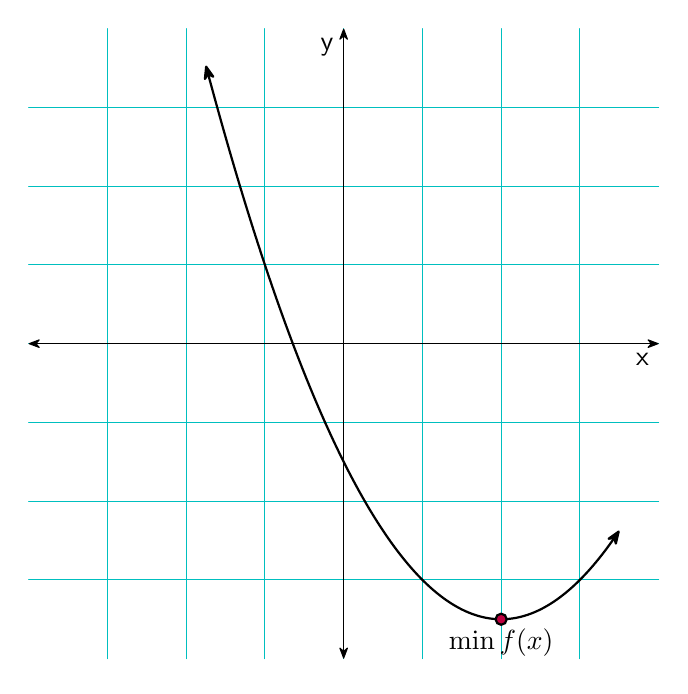
\begin{tikzpicture}

\foreach \i in {-3,...,3}
    \draw[line cap = round, Cyan!75!Black] (\i, -4) -- (\i, 4) %
    (-4, \i) -- (4, \i);

\draw[{Stealth[round]}-{Stealth[round]}] (-4,0) -- (4,0);
\draw[{Stealth[round]}-{Stealth[round]}] (0, -4) -- (0, 4);

\node at (4, 0) [anchor=north east] {$\mathsf{x}$};
\node at (0, 4) [anchor=north east] {$\mathsf{y}$};

\begin{axis}[axis x line=none,axis y line=none,xticklabels=\empty,yticklabels=\empty,xmin=-4, xmax=4,ymin=-4, ymax=4, xshift=-4cm, yshift=-4cm, x=1cm,  y=1cm]

    \addplot [thick, line cap=round, samples=500, domain=-1.75:3.5, {Stealth[round]}-{Stealth[round]}] {0.5*x^2 - 2*x -1.5};

\end{axis}

\node at (2, -3.5) [anchor=north] {$\min{f(x)}$};
\draw[thick, fill=purple] (2, -3.5) circle (2pt);
\end{tikzpicture}
\end{document}
